\documentclass[../../../thesis.tex]{subfiles}

\begin{document}
  \begin{figure}[ht]
		\centering
    \tikzsetnextfilename{pshift}
    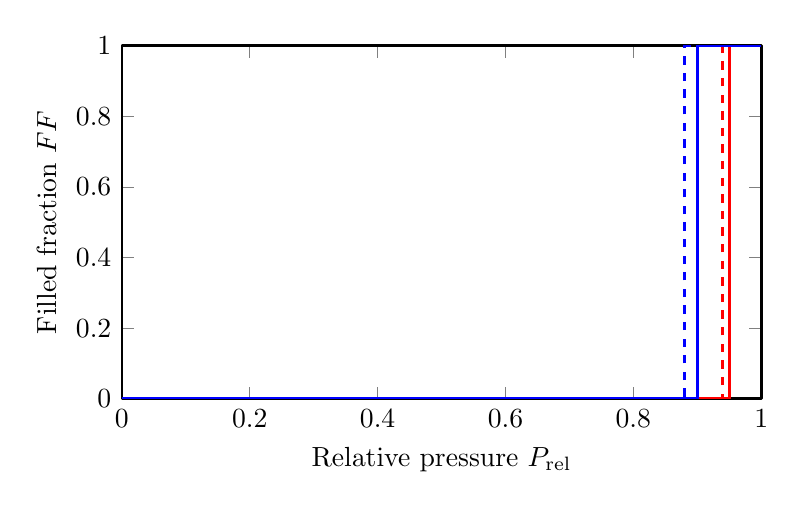
\begin{tikzpicture}
        \begin{axis}[
          /tikz/line join=bevel,
          width=0.8*\textwidth,
          height=0.5*\textwidth,
          legend style={at={(0,.5)}, legend columns=1, anchor=south west},
          every axis plot,
					line width = 1pt,
					xmin = 0, xmax = 1,
					ymin = 0, ymax = 1,,
					xlabel = {Relative pressure $P_\mathrm{rel}$},
					ylabel = {Filled fraction $FF$},
          ]
					% Add plots
          \addplot [color=red, mark=none]
            coordinates {
            (0, 0)
            (.95,0)
            (.95,1)
            (1,1)};
          \addplot [color=red, mark=none, dashed]
            coordinates {
            (0, 0)
            (.94,0)
            (.94,1)
            (1,1)};
            \addplot [color=blue, mark=none]
              coordinates {
              (0, 0)
              (.9,0)
              (.9,1)
              (1,1)};
            \addplot [color=blue, mark=none, dashed]
              coordinates {
              (0,0)
              (.88,0)
              (.88,1)
              (1,1)};
        \end{axis}
    \end{tikzpicture}
    \label{fig:pshift}
    \caption{Shift of the condensation and evaporation pressure to lower values due to the reduction of the effective pore diameter.}
  \end{figure}
\end{document}
